\documentclass[a4paper,11pt]{article}

\usepackage{cite}
\usepackage[T1]{fontenc}
\usepackage[utf8]{inputenc}
\usepackage{graphicx}
\usepackage{fancyheadings}
\usepackage{geometry}
\usepackage{multicol}
\usepackage{amsmath}
\usepackage{amssymb}
\usepackage{pdfpages}
\usepackage{caption} 
\usepackage[]{algorithm2e}

\captionsetup[table]{skip=10pt}

 \newcommand{\ba}[1]{\begin{align*}    #1    \end{align*}}
 \newcommand{\ban}[1]{\begin{align}    #1    \end{align}}
 \renewcommand{\vec}[1]{\mathbf{#1}}
 \newcommand{\bothset}[3]{\overset{#2}{\underset{#3}{#1}}}

 \definecolor{light-gray}{gray}{0.95}

\setlength{\headsep}{1in}

\pagestyle{fancy}

\lhead{ridenour@kth.se \\ herczka@kth.se}
\rhead{Parallel Programming for Large-Scale Problems SF2568}
\title{ Analysis of a Parallel Solver for the Gray-Scott Reaction-Diffusion System\\ 
\vspace{1.2cm}
\large Parallel Programming for Large-Scale Problems SF2568 \\ 
Teacher: Michael Hanke}
\author{Jonathan Ridenour, 780514-7779\\
Mateusz Herczka, 700624-9234}

\begin{document}
\maketitle
\pagebreak
\section*{Problem description}
The subject of this report is the parallelisation of a numerical method for a two-component reaction-diffusion system known as the Gray-Scott model.  Originally introduced by Gray and Scott \cite{Gray}, the model is a system of two partial differential equations for the concentration of two chemical species, which are reacting with each other as they diffuse through a medium.

Pattern formation resulting from the Gray-Scott model is a rich area of research, with applications to a variety of physical, chemical, and biological phenomena, as well as cellular automata and the pattern formation of other partial differential equation systems \cite{Wang}.  We investigate a parallelisation strategy for the two-dimensional case.  We make a series of trials, running the solver in parallel on 4, 16, 64, and 100 processes, and perform a speedup analysis using the results of these trials. Finally, we show a few of the various patterns that emerge from the Gray-Scott model with various input parameters.

\subsection*{Mathematical Formulation}
The Gray-Scott model involves the reaction and diffusion of two generic chemical species, $U$ and $V$, whose concentrations are described by the functions $u$ and $v$, reacting according to the chemical equations
\ba{
U + 2V \rightarrow  & \ 3V,\\
V \rightarrow  & \ P,
}
where $P$ is an inert byproduct.  This system is governed by the following system of partial differential equations, known as the Gray-Scott equations:
\begingroup
\addtolength{\jot}{0.5 em}
\ban{
\label{eq:gsu}
\frac{\partial u}{\partial t} = & \ D_u \nabla^2u - uv^2 + F(1-u), & \ u,v: \Omega \mapsto \mathbb{R}, \ t\ge 0,  \\
\label{eq:gsv}
\frac{\partial v}{\partial t} = & \ D_v \nabla^2v + uv^2 - (F-K)v , & \ u,v: \Omega \mapsto \mathbb{R}, t \ \ge 0.
}
\endgroup
Here, $D_u$ and $D_v$ are the diffusion constants for $u$ and $v$ respectively, and $F$ and $K$ are constants which govern the replenishment of the chemical species.  The term $uv^2$ gives the reaction rate for the system.  We are concerned with solving the Gray-Scott equations on a two-dimensional domain $\Omega = [0,1]^2$.  Thus, $u = u(x,y,t)$ and $v = v(x,y,t)$, giving the laplacian as
\ba{
\nabla^2u = & \ \frac{\partial^2 u}{\partial x^2} + \frac{\partial^2 u}{\partial y^2}, \\
\nabla^2u = & \ \frac{\partial^2 u}{\partial x^2} + \frac{\partial^2 u}{\partial y^2}.
}

As in \cite{Wang}, we use periodic boundary conditions for (\ref{eq:gsu}) and (\ref{eq:gsv}); thus, our simulation on $\Omega$ models a small surface surrounded by similar elements reacting identically. We choose the diffusion constants $D_u = 2 \cdot 10^{-6}$, $D_v = 1 \cdot 10^{-6}$, and let $F$ and $K$ take values according to $F \in [0.02, \ 0.08]$, $K \in [0.05,\ 0.07]$ in order to investigate the different types of patterns that arise from varying combinations of the two.

The system is in a trivial state when $u = 1$ and $v=0$.  To initialize a reaction, we let the system assume this trivial state at time zero in all areas except a square in the middle of dimension one-sixth, where we set $u = 0.5$ and $v = 0.25$:
\ban{
\label{eq:icu}
u(x,y,0) = \begin{cases}
1/2, & \ 5/12 \ge x \ge 7/12, \ 5/12 \ge y \ge 7/12,\\
1, & \ \text{otherwise},
 \end{cases}\\
 \label{eq:icv}
 v(x,y,0) = \begin{cases}
1/4, & \ 5/12 \ge x \ge 7/12, \ 5/12 \ge y \ge 7/12,\\
0, & \ \text{otherwise}.
 \end{cases}
}
The reaction then diffuses outward from the middle, leaving behind a characteristic pattern, until all $\Omega$ is filled.

\subsection*{Numerical Method}
We discretize $\Omega$ with the same stepsize in the $x$- and $y$-directions, $h$, corresponding to $N^2$ inner gridpoints equidistantly spread across the surface.  We let $h = 1/(N+1)$ such that $x_i = ih$, $i$ = 1, 2, . . . , $N$ and $y_j = jh$, $j$ = 1, 2, . . . , $N$.  Thus the function value $u(x,y,t)$ is approximated by $u(ih, jh, t) = u_{i,j}(t)$, $t\ge 0$. Using the traditional central difference formula for the discrete five-point laplacian with step length $h$, $\Delta_5^h$, the system (\ref{eq:gsu}) + (\ref{eq:gsv}) can be written in semi-discrete form as follows: 
\begingroup
\addtolength{\jot}{0.5 em}
\ban{
\label{eq:semiu}
\frac{\partial u_{i,j}}{\partial t} = \frac{D_u}{h^2} \Delta_5^h u_{i,j} -u_{i,j} (v_{i,j})^2 + F(1-u_{i,j}), \\
\label{eq:semiv}
\frac{\partial v_{i,j}}{\partial t} = \frac{D_v}{h^2} \Delta_5^h v_{i,j} +u_{i,j} (v_{i,j})^2 - (F-K)v_{i,j}.
}
\endgroup
We then discretize in time, with timestep $dt$, and approximate the time-derivative with the explicit Euler method.  Letting $t = k\cdot dt$ for $k$ = 1, 2, 3, . . . ., and $u_{i,j}(k\cdot dt) = u_{i,j}^k$, $v_{i,j}(k\cdot dt) = v_{i,j}^k$, the system (\ref{eq:semiu}) + (\ref{eq:semiv})  becomes
\begingroup
\addtolength{\jot}{0.5 em}
\ban{
\label{eq:difu}
\frac{u_{i,j}^{k+1} - u_{i,j}^k}{dt} = \frac{D_u}{h^2} \Delta_5^h u_{i,j}^k -u_{i,j}^k (v_{i,j}^k)^2 + F(1-u_{i,j}^k), \\
\label{eq:difv}
\frac{v_{i,j}^{k+1} - v_{i,j}^k}{dt} = \frac{D_v}{h^2} \Delta_5^h v_{i,j}^k +u_{i,j}^k (v_{i,j}^k)^2 - (F-K)v_{i,j}^k.
}
\endgroup
The difference equations (\ref{eq:difu}) and (\ref{eq:difv}) give a simple formula for the update of the function values at time $(k+1) \cdot dt$ given that values at time $k \cdot dt$.  We represent the discrete functions $u_{i,j}^k$ and  $v_{i,j}^k$ as long vectors $\vec{u}^k$ and $\vec{v}^k$ with the following enumeration:
\ba{
\vec{u}^k = & \ (u_{1,1}^k, \ u_{2,1}^k, \ \text{. . . }, \ u_{N,1}^k, \ u_{1,2}^k, \ u_{2,2}^k, \ \text{. . . }, \ u_{N,N}^k), \\
\vec{v}^k = & \ (v_{1,1}^k, \ v_{2,1}^k, \ \text{. . . }, \ v_{N,1}^k, \ v_{1,2}^k, \ v_{2,2}^k, \ \text{. . . }, \ v_{N,N}^k).
}
Using the long vectors, we can write the numerical operator $\Delta_5^h$ as a sparse matrix multiplication as follows:
\begingroup
\addtolength{\jot}{0.5 em}
\ba{
\frac{D_u}{h^2} \Delta_5^h u_{i,j} = \vec{A}_u\vec{u}^n,\\
\frac{D_v}{h^2} \Delta_5^h v_{i,j} = \vec{A}_v\vec{v}^n,
}
\endgroup
where the matrices $\vec{A}_u$ and $\vec{A}_v$ are of dimension $[N^2 \times N^2]$ with block tridiagonal form:
\ba{
\vec{A}_u = & \ \text{tridiag}_N(\sigma_u\vec{I}, \ \vec{T}_u, \ \sigma_u\vec{I}), \\
\vec{A}_v = & \ \text{tridiag}_N(\sigma_v\vec{I}, \ \vec{T}_v, \ \sigma_v\vec{I}),
}
where $\vec{I}$ is an identity matrix, multiplied by the constants $\sigma_u$ or $\sigma_v$, and the matrices $\vec{T}_u$ and $\vec{T}_v$ are tridiagonal of the form
\ba{
\vec{T}_u = & \ \text{tridiag}_N(\sigma_u, \ -4\sigma_u, \ \sigma_u), \\
\vec{T}_v = & \ \text{tridiag}_N(\sigma_v, \ -4\sigma_v, \ \sigma_v),
}
where 
\begingroup
\addtolength{\jot}{0.5em}
\ba{
\sigma_u =& \ \frac{D_u}{h^2}, \\
\sigma_v =& \ \frac{D_v}{h^2}.
}
\endgroup
If we let $f_u(\vec{u}^{k},\vec{v}^{k}) = -\vec{u}^k (\vec{v}^k)^2 + F(1-\vec{u}^k)$ and $ f_v(\vec{u}^{k},\vec{v}^{k}) = \vec{u}^k (\vec{v}^k)^2 - (F-k)\vec{v}^k$, we can compactly write the fully discretized equations as
\ban{
\label{eq:discu}
\vec{u}^{k+1} = \vec{u}^{k} + dt [\vec{A}_u \vec{u}^{k} + f_u(\vec{u}^{k},\vec{v}^{k})],\\
\label{eq:discv}
\vec{v}^{k+1} = \vec{v}^{k} + dt [\vec{A}_v \vec{v}^{k} + f_v(\vec{u}^{k},\vec{v}^{k})],
}
and we have an exact update formula for each time step.
\subsubsection*{Initial and Boundary Conditions}
The initial and boundary conditions are straightforward to implement numerically.  The initial state is completely known, so $\vec{u}^0$ and $\vec{v}^0$ are given.  To implement periodic boundary conditions we simply set
\ba{
u_{-1,j}^k = & \ u_{N-1,j}^k, \\
u_{i,-1}^k =& \  u_{i,N-1}^k, \\
u_{N,j}^k =& \  u_{0,j}^k,\\ 
u_{i,N}^k = & \ u_{i,0}^k,\\ 
}
when updating the boundary points.  The formula is likewise for $v$.

\subsubsection*{Stability Conditions}
In order to ensure numerical stability for the differential operators $\vec{A}_u$ and $\vec{A}_v$ in  (\ref{eq:discu}) and (\ref{eq:discv}), we must conform to the restriction
\ba{
dt \cdot \lambda_{l,u} \in & \ \mathcal{S}, \ \forall  \ l, \ l = \text{1, 2, . . . $L_u$},\\
dt \cdot \lambda_{l,v} \in & \ \mathcal{S}, \ \forall  \ l, \ l = \text{1, 2, . . . $L_v$},
}
where $\lambda_{l,u}$ and $\lambda_{l,v}$ are the $l$-th eigenvalues of $\vec{A}_u$ and $\vec{A}_v$ respectively,  and $\mathcal{S}$ is the stability region of the explicit Euler method: a circle in the complex plane centered at $-1$ with unit radius \cite{Edsberg}.  The number of unique eigenvalues possessed by each of the matrices is denoted by $L_u$ and $L_v$.   

For the parallel speedup trials, we discretize $\Omega$ using $N = 400$.  Together with the chosen diffusion constants, the  maximum eigenvalue, $\lambda_{max}$, of $\vec{A}_u$ and $\vec{A}_v$ has a strictly negative real value, and thus we must choose a timestep such that $dt \cdot \lambda_{max}$ is at least $-2$.  The maximum eigenvalue is computed using Matlab as:
\ba{
\lambda_{max} = -1.2735,
}
which provides the limitation on the timestep:
\ba{
dt \le \frac{-2}{-1.2735} = 1.5704.
}
Since the timestep also has a damping effect on the replenishment term and reaction rate, we must consider these as well when choosing the timestep.  As in \cite{Wang}, we settle on a value which is comfortably beneath the max:
\ba{
dt = 0.75.
}
This is well within the stability bounds imposed by $\vec{A}_u$ and $\vec{A}_v$; it also provides suitable damping on the replenishment and reaction rate terms for the observation of the characteristic Gray-Scott pattern formation.

\section*{Algorithm Description}
\subsection*{Implementation details}
To implement the update formulae (\ref{eq:discu}) and (\ref{eq:discv}) in parallel, the computational domain is divided into subdomains, one for each process.  Each process is responsible for the update of it's local values.  Along the subdomain boundaries, neighbouring values are needed for the update; these are obtained by coordinated message-passing.  The boundary data are communicated between processes by means of a red-black communication schedule.  When all necessary information is obtained, the local values are updated according to (\ref{eq:discu}) and (\ref{eq:discv}), see Algorithm \ref{alg:coms}.

For a domain size of $400 \times 400$, the global update boils down to two matrix multiplications, one using $\vec{A}_u$, one using $\vec{A}_v$, each of which contains $400^4$ elements, most of which are zero.  This can be accomplished by means of a sparse matrix multiplication method, or direct kernel computations. First we describe their common structure.

The 5-point computation molecule is dependent on four neighbours labeled NORTH, EAST, SOUTH and WEST. We define a 2D cartesian mesh of pxp processes, where p = sqrt(P). The NxN domain is decomposed into P square subdomains, each with dimension nxn elements, where n = sqrt(N). The challenge becomes to communicate the domain borders between neighbours, and synchronize this with computation of the domain interior. We implement a red-black scheme as follows:

\vspace{0.7 cm}
\begin{algorithm}[H]
  \SetAlgoLined
  \eIf{(even row AND even process) OR (odd row AND odd process)}{
    color := red\;
  }{
    \tcc*[h]{(even row AND odd process) OR (odd row AND even process)}
    color := black\;
  }
  \caption{Determining process color}
\end{algorithm}
\vspace{0.7 cm}

The 2D process grid is thus colored in a checkerboard pattern. Since we use periodic boundary conditions, we assume even p to ensure red-black neighbours when wrapping around the boundaries of the grid. Because the subdomain borders are shared between neighbours, we implement overlap by introducing a ghost frame surrounding the subdomain, labeled GHOST\textunderscore NORTH, GHOST\textunderscore EAST, GHOST\textunderscore SOUTH and GHOST\textunderscore WEST, which give each subdomain a total dimension of (n+2)x(n+2). In addition, we define four borders of the inner nxn domain, labeled BORDER\textunderscore NORTH, BORDER\textunderscore EAST etc. The values in the borders are recalculated every iteration, then sent to the corresponding neighbour. The values in the ghosts are used when the computation molecule centers on an element at a border. They are received from a neighbour every iteration before the computation phase starts.

Each computation iteration is preceded by a communication phase arranged in four parts to avoid deadlock. Each sendreceive is done once for u and once for v. We also show the timing calls:

\vspace{0.7 cm}
\begin{algorithm}[H]
  \SetAlgoLined
  \While{iter < maxiter}
  {
    start := startTimer()\;
    \eIf{(red)}{
      \tcc*[h]{paramlist (sendbuffer, receivebuffer, neighbour)}\\
      sendreceive(BORDER\textunderscore NORTH, GHOST\textunderscore NORTH, neighbour[NORTH])\;
      sendreceive(BORDER\textunderscore SOUTH, GHOST\textunderscore SOUTH, neighbour[SOUTH])\;
      sendreceive(BORDER\textunderscore EAST, GHOST\textunderscore EAST, neighbour[EAST])\; 
      sendreceive(BORDER\textunderscore WEST, GHOST\textunderscore WEST, neighbour[WEST])\; 
    }{
      \tcc*[h]{black}\\
      sendreceive(BORDER\textunderscore SOUTH, GHOST\textunderscore SOUTH, neighbour[SOUTH])\;
      sendreceive(BORDER\textunderscore NORTH, GHOST\textunderscore NORTH, neighbour[NORTH])\;  
      sendreceive(BORDER\textunderscore WEST, GHOST\textunderscore WEST, neighbour[WEST])\;
      sendreceive(BORDER\textunderscore EAST, GHOST\textunderscore EAST, neighbour[EAST])\;
    }
    end := endTimer()\;
    tComm += end-start\;
    start := startTimer()\;   
    calculateDomain()\;
    end := endTimer()\;
    tCalc += end-start\;
    iter++\;
  }
  \caption{Sendreceive phases with timing calls}
\end{algorithm}
\vspace{0.7 cm}

We now describe the specifics our two implementations, which differ mainly in the calculateDomain() procedure. The matrix version uses a small sparse matrix library called CSparse, which accompanies ``Direct Methods for Sparse Linear Systems'' [#reference#]. The author, who has contributed to several matrix routines in MATLAB as well as NVIDIA, describes CSparse as ``for educational use''. While fast, it's not fully competitive with professional libraries. Yet the code is readable and enables us to formulate code similar to MATLAB and formulas (9) and (10). CSparse doesn't reference any other libraries, so the code is portable between our laptops and Ferlin. We show only the expressions for u, with v being analogous:

\vspace{0.7 cm}
\begin{algorithm}[H]
  \SetAlgoLined
  \ForEach{element $i$ in $u$}{
    unew[i] = u[i] + ht * ( (-u[i] * v[i]^2) + (F * (1.0 - u[i])) )\;

    \tcc*[h]{CSparse call equivalent to: unew = Au*v + unew,}\\

    \tcc*[h]{where Au is a constant, sparse matrix.}\\ 

    csGaxpy(Au, u, unew)\;
    unew[boundaries] += sigma * ghost\;
    }
  \caption{Sparse matrix implementation of calculateDomain()}
\end{algorithm}
\vspace{0.7 cm}


The east and west borders/ghosts are columns and thus non-contiguous in memory. This version maintains two work buffers for this data, which is arranged sequentially and copied into these buffers before IO. While 

The kernel version computes the 5-point molecule for each domain element with a direct expression:

def calculateDomain():

  ru = (ht * DU) / hx^2

  for each i,j in domain

    unew[i][j] = u[i][j] + ru * (u[i - 1][j] - (4 * u[i][j]) + u[i + 1][j] + u[i][j - 1] + u[i][j + 1]) + ht * (-u[i][j] * v[i][j] * v[i][j] + F * (1.0 - u[i][j]))

  end for

end

Also, in the kernel implementation we make use of more mpi routines. We use MPI_Cart functions to set up an mpi process mesh. This allows for defining arrays of neighbour coordinates, including diagonals for future use with a 9-point kernel. This setup is also easy to extend into 3D. For the east and west column borders, we define MPI_Type_vector's which omit the buffer copying.

Finally, our programs save the domains as matrix blocks which are automatically assembled and plotted in MATLAB.



\vspace{0.7 cm}
\begin{algorithm}[H]
\label{alg:coms}
 \KwData{$dt$, $\vec{u}^k$, $\vec{v}^k$, $\vec{A}_u$, $\vec{A}_v$, red}
 \KwResult{$\vec{u}^{k+1}$ and $\vec{v}^{k+1}$ }
collect boundary data $\vec{b}_{out}$\;
  \eIf{red}{
send $\vec{b}_{out}$: north, south, east, west\;
receive $\vec{b}_{in}$: south, north, west, east\;
   }{
receive $\vec{b}_{in}$: south, north, west, east\;
send $\vec{b}_{out}$: north, south, east, west\;
  }
$\vec{u}^{k+1} = \vec{u}^k+ dt [\vec{A}_u \vec{u}^k +  f_u(\vec{u}^{k},\vec{v}^{k})] + \vec{b}_{in}$\;
$\vec{v}^{k+1} = \vec{v}^k+ dt [\vec{A}_v \vec{v}^k +  f_v(\vec{u}^{k},\vec{v}^{k})] + \vec{b}_{in}$\;
 \vspace{0.3 cm}
\caption{Communication and local update.}
\end{algorithm}
\vspace{0.7 cm}

\section*{Performance Evaluation}
\subsection*{Extrapolated Speedup}
In an attempt to predict the parallel speedup we can expect to achieve as we increase the number of processes, we perform an initial run on 1 and 4 processes, compute the speedup $S_4$, and extrapolate to $S_P$ using Amdahl's Law.  For the test case employing sparse matrix multiplication, we get an run time of 793.15 s on one process, and 304.39 s on 4 processes.  This gives the initial speedup:
\ba{
S_4 = \frac{T_1}{T_4} = 2.606.
}
Using Amdahl's Law we can solve for $f$, the fraction of the computation which cannot be divided into parallel tasks:
\ba{
S_4 = \frac{4}{1+3f} \Rightarrow f = \frac{4-S_4}{3S_4} = 0.1783.
}
Applying this same analysis to the kernel method, we get the following calculation:
\ba{
S_4 = \frac{T_1}{T_4} = \frac{113.0}{94.26} =  1.199 \Rightarrow f = \frac{4-S_4}{3S_4} = 0.7789.
}
Table \ref{tab:S_extrap} shows the extrapolated speedup that these values for $f$ indicate for 16, 64, and 100 processes.  This method is obviously a poor predictor for both the parallelisation strategies we employ.  Indeed, our experimental speedup trials indicate that the problem scales very well on increased numbers of processes, see figures \ref{fig:sparse} and \ref{fig:kernel}.

\begin{table}[h]
\def\arraystretch{1.2}
\begin{center}
\caption{Extrapolated speedup given by Amdahl's Law.}
\label{tab:S_extrap}
%\vspace{0.1cm}
\begin{tabular}{| l | c | c | c | c | c |}
\hline
&$P$ & 4 & 16 & 64 & 100 \\
\hline
Sparse matrix method & $S_P $& 2.6 & 4.3 & 5.2 & 5.4\\
\hline
Kernal method & $S_P $& 1.2 & 1.3 & 1.3 & 1.3\\
\hline
\end{tabular}
\end{center}
\end{table}

\subsection*{Experimental Speedup}
We run a series of trials on Ferlin and record the initialisation time, $t_{init}$, the communication time, $t_{comm}$, the calculation time, $t_{calc}$, and the total run time $t_{tot}$.  Tables \ref{tab:matrix} and \ref{tab:kernal} show the maximum of these values for each of the trials at 1, 4, 16, 64, and 100 processes.  The values of $t_{tot}$ are used to compute the experimental speedup, shown in figures \ref{fig:sparse} and \ref{fig:kernel}.

\begin{table}[h]
\def\arraystretch{1.2}
\begin{center}
\caption{Max time (seconds) measurements, sparse matrix method.}
\label{tab:matrix}
%\vspace{0.3cm}
\begin{tabular}{| c | c | c | c | c |}
\hline
$P$ & $t_{init}$ & $t_{comm}$ & $t_{calc}$ & $t_{tot}$ \\
\hline
1 & 0.1437 &  0.000 & 793.0 & 703.14\\
\hline
4 & 0.05663 & 36.48 & 301.8 & 304.4\\
\hline
16 & 0.008907 & 8.786 & 38.42 & 40.87\\
\hline
64 & 0.009324 & 2.8460 & 7.391 & 9.603\\
\hline
100 & 0.001253 & 3.206 & 4.287 & 7.419\\
\hline
\end{tabular}
\end{center}
\end{table}

\begin{table}[h]
\def\arraystretch{1.2}
\begin{center}
\caption{Max time (seconds) measurements, kernel method.}
\label{tab:kernal}
%\vspace{0.3cm}
\begin{tabular}{| c | c | c | c | c |}
\hline
$P$ & $t_{init}$ & $t_{comm}$ & $t_{calc}$ & $t_{tot}$ \\
\hline
1 & 0.0046 & 0.0000 &113.0 &113.0\\
\hline
4 & 0.0051& 3.157 & 91.37 & 94.26\\
\hline
16 & 0.1540 & 3.115 & 6.559 & 9.778\\
\hline
64 & 0.1845 & 2.410 &1.683 &4.248 \\
\hline
100 &1.197 & 3.293 & 1.081 & 5.556 \\
\hline
\end{tabular}
\end{center}
\end{table}

\begin{figure}
  \centering
  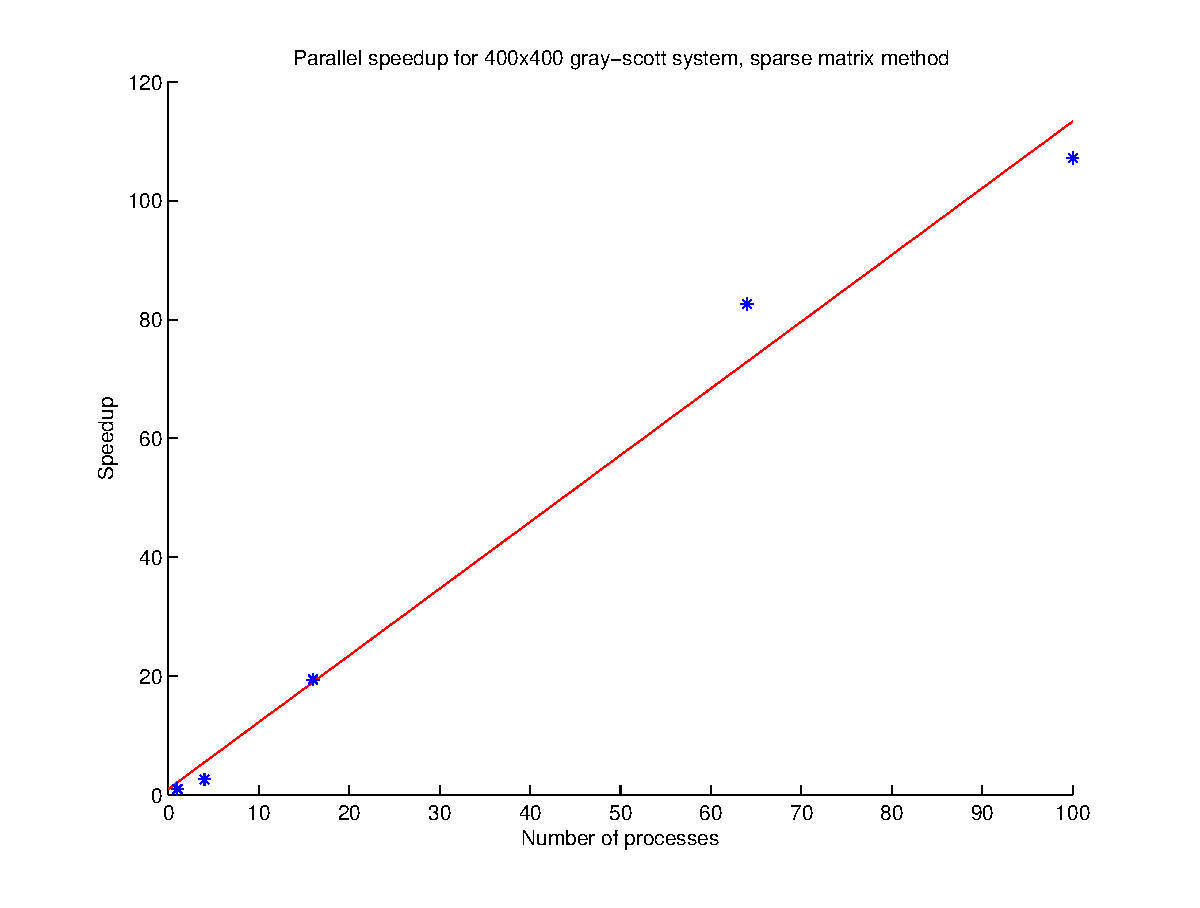
\includegraphics[scale=0.6]{sparse}
    \caption{Experimental speedup, sparse matrix multiplication method.}
    \label{fig:sparse}
\end{figure}

\begin{figure}
  \centering
  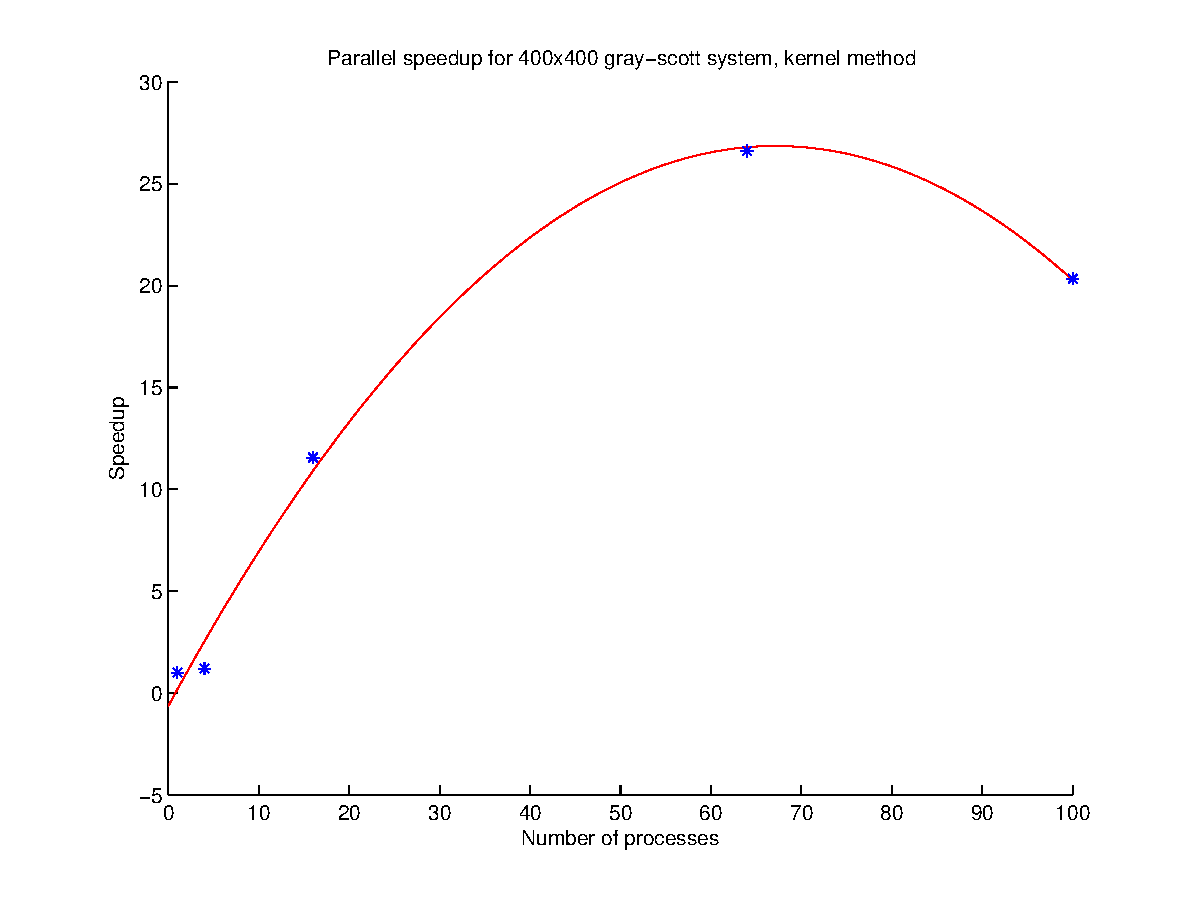
\includegraphics[scale=0.6]{kernel}
    \caption{Experimental speedup, kernel method.}
    \label{fig:kernel}
\end{figure}

\subsection*{Larger Domain}
Using the faster kernel method, we conduct another numerical experiment on Ferlin with a 1000x1000 domain and same number of iterations. We find that dt = 0.075 is sufficient for stability, while still yielding a pattern growth which almost fills the entire domain. As before, we run 1, 4, 16, 64, and 100 processes. 

\begin{table}[h]
\def\arraystretch{1.2}
\begin{center}
\caption{Max time (seconds) measurements, kernel method, 1000x1000 domain.}
\label{tab:matrix}
%\vspace{0.3cm}
\begin{tabular}{| c | c | c | c | c |}
\hline
$P$ & $t_{init}$ & $t_{comm}$ & $t_{calc}$ & $t_{tot}$ \\
\hline
1 & 0.02936 &  0.000 & 756.86 & 756.89\\
\hline
4 & 0.00555 & 71.502 & 398.283 & 469.79\\
\hline
16 & 0.06474 & 14.1897 & 47.0218 & 61.276\\
\hline
64 & 0.1676 & 11.099 & 17.286 & 28.553\\
\hline
100 & 1.1956 & 10.215 & 6.5125 & 17.923\\
\hline
\end{tabular}
\end{center}
\end{table}

\begin{figure}
  \centering
  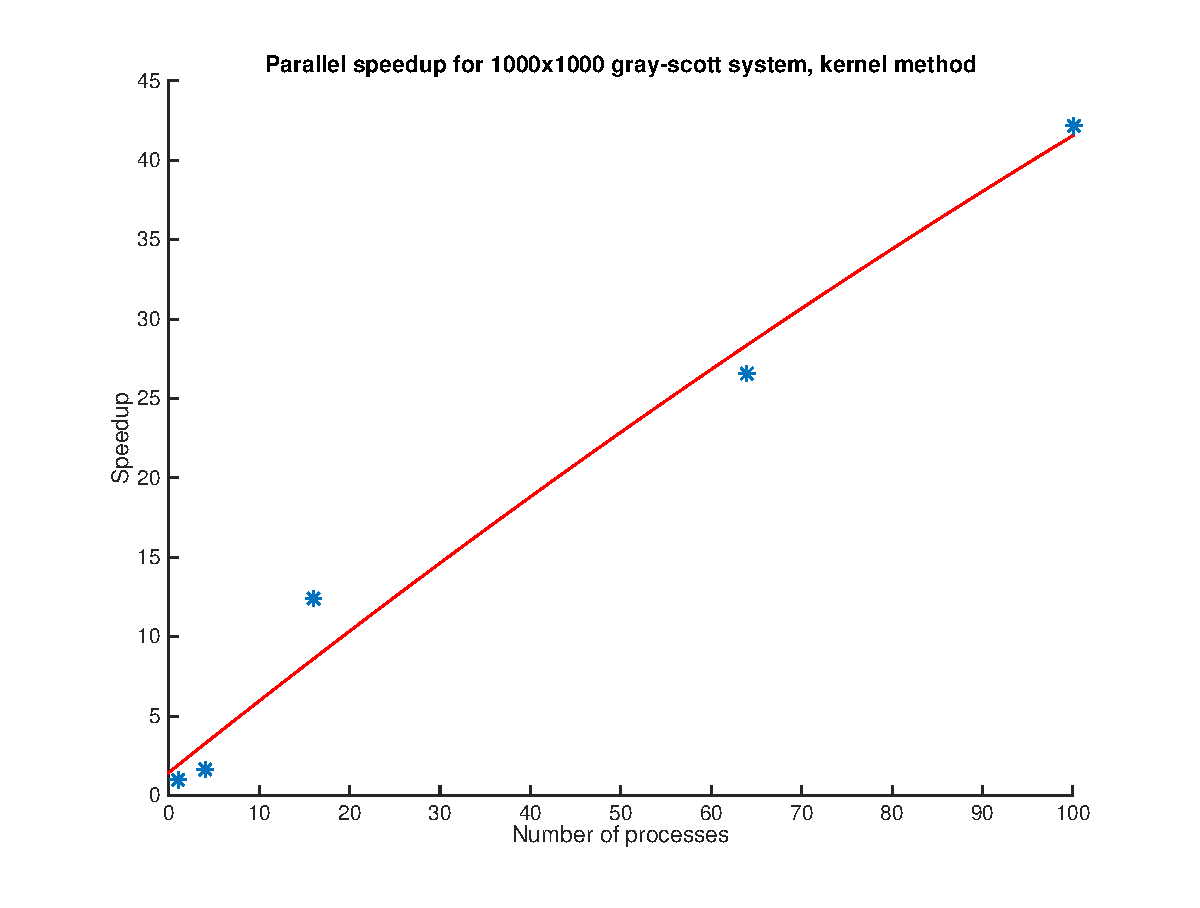
\includegraphics[scale=0.6]{kernel-1k}
    \caption{Experimental speedup, kernel method, 1000x1000 domain.}
    \label{fig:kernel-1k}
\end{figure}

\subsection*{Speedup Analysis}
There are a few reasons why the extrapolation of Amdahl's Law does not provide an accurate predictor for the parallel speedup.  The most obvious reason is that $f$, the fraction of the computation which cannot be divided into parallel tasks, does not in itself account for an upper bound on the speedup.  In fact, our best measure of $f$ is $t_{init}$ and, as can be seen in tables \ref{tab:matrix} and \ref{tab:kernal}, this accounts for only a minuscule portion of the total runtime.  It is more likely that the speedup can be explained by the memory hierarchies employed by Ferlin.  

** TVEKSAMT vi vet inget om hur ferlin är byggd. When the number of processes is low, so is the available cache.  As the number of processes increases, more of the working set, and at some point the entire working set, can fit into the available caches, allowing for a quicker memory access time. **

The matrix implementation shows a mostly linear speedup (although the plot could be interpreted as a gently decreasing curve), but the sequential version is not fast. We suspect that the sparse matrix multiplication largely fails to exploit memory proximity, and a large fraction of memory accesses result in a cache miss. On the other hand, the kernel implementation (which is several times faster both sequentially and in parallel), accesses memory in a linear fashion more favorable for caching. Looking at its initially supralinear speedup which sharply descends after 64 processes, we suspect that there exists (for this computer) an optimal domain size per node. We conclude that profiling is essential for optimal code design.

\section*{Patterns}
\section*{Conclusions}

\clearpage
\begin{thebibliography}{}
\bibitem{Gray} Gray P, Scott SK. {\it Sustained oscillations and other exotic patterns of behavior in isothermal reactions}. J Phys Chem 1985;89:22–32.
\bibitem{Wang} Weiming Wang, Yezhi Lin, Feng Yang, Lei Zhang, Yongji Tan, {\it Numerical study of pattern formation in an extended Gray–Scott model}, Communications in Nonlinear Science and Numerical Simulation, 16 (2011).
%\bibitem{Ruuth} Steven J Ruuth, {\it Implicit-Explicit Methods for Reaction-Diffusion Problems in Pattern Formation}, Journal of Mathematical Biology 34 (2), 148-176. 
\bibitem{Edsberg} Lennart Edsberg {\it Introduction to Computation and Modelling for Differential Equations}, 2008, John Wiley and Sons, pp 50.
%\bibitem{Wilkinson} Barry Wilkinson, Michael Allen {\it Parallel Programming, Techniques and Applications Using Networked Workstations and Parallel Computers}, 2005, Pearson Prentice Hall, pp 9.
\end{thebibliography}

\end{document}